\documentclass[main.tex]{subfiles}
\begin{document}
    %\addtocontents{toc}{\protect\newpage}

    \chapter{Dynamics}
        \label{ch: Dynamics}
        \thispagestyle{noheader}

        Dynamics is the study of forces and how they give rise to motion.


        \section{Base Units}
            \label{sec: Base Units Dynamics}

            \begin{table}[!h]
                \noindent\begin{tabular}{@{} p{40mm} C{10mm} p{110mm}}
                    Mass &($m$) &Kilogram (\si{\kilo\gram})\\[\tablegap]
                    Distance &($s$) &Metres (\si{\metre})\\[\tablegap]
                    Displacement &($\vect{s}$) &Metres (\si{\metre})\\[\tablegap]
                    Time &($t$) &Seconds (\si{\second})\\[\tablegap]
                    Speed &($v$) &Metres per Second (\si{\metre \per\second} \textbf{or} \si{\metre / \second})\\[\tablegap]
                    Velocity &($\vect{v}$) &Metres per Second (\si{\metre \per\second} \textbf{or} \si{\metre / \second})\\[\tablegap]
                    Acceleration &($\vect{a}$) &Metres per Second, per Second (\si{\metre \per\second\squared} \textbf{or} \si{\metre /\second /\second} \textbf{or} \si{\metre / \second\squared})\\[\tablegap]
                    Force &($\vect{F}$) &Newtons (\si{\newton}) \textbf{or} (\si{\kilo\gram \metre \per\second\squared})\\[\tablegap]
                    Energy &($E$) &Joules (\si{\joule}) \textbf{or} (\si{\kilo\gram \metre\squared \per\second\squared})\\[\tablegap]
                    Work &($W$) &Joules (\si{\joule}) \textbf{or} (\si{\newton \metre}) \textbf{or} (\si{\kilo\gram \metre\squared \per\second\squared})\\[\tablegap]
                    Power &($P$) &Joules per second (\si{\joule \per\second}) \textbf{or} (\si{\kilo\gram \metre\squared \per\second\cubed})
                \end{tabular}
            \end{table}



        \section{Constants}
            \label{sec: Constants Dynamics}

            Gravitational acceleration at Earth's surface ($g$) -- $9.8\ m\,s^{-2}$
            



        \section{Equations}
            \label{sec: Equations Dynamics}

            \begin{fleqn}
                \begin{align}
                    \vect{F}_{net} = m\vect{a}
                    \label{eq: Net Force}
                \end{align}
                \eqexp{The equation describing the relationship between the net force on an object and the acceleration on an object with constant mass.\\The net force is found by adding all of the force vectors on an object (important because you cannot just add the magnitudes).}

                \begin{align}
                    \vect{p} = m \vect{v}
                \end{align}
                \eqexp{The momentum of an object.}


                \newpage


                \begin{align}
                    I = \vect{F} \Delta t = \Delta \vect{p}
                \end{align}

                \eqexp{Impulse is the change in momentum due to a force over some (usually small) time.}
                
                
                \begin{align}
                    f_k &= \mu_k N
                    \label{eq: Kinetic Friction}\\
                    f_s &\leq \mu_s N
                    \label{eq: Static Friction}
                \end{align}
                \eqexp{The equations describing the strength of the friction force between two objects.\\$f_k$ describes the kinetic friction which is present when the objects are sliding across each other.\\$f_s$ describes the upper limit on the static friction force which occurs when two objects are not moving relative to each other but have other forces trying to slide them across each other.}


                \begin{align}
                    E_k = \frac{1}{2}m v^2
                    \label{eq: Kinetic Energy}
                \end{align}
                \eqexp{The kinetic energy of an object with mass $m$ and speed $v$.}


                \begin{align}
                    W = \Delta E_k
                    \label{eq: Work as Change in Kinetic Energy}
                \end{align}
                \eqexp{The work done on an object describes it's change in kinetic energy.}


                \begin{align}
                    W_A = \vect{F}_A\cdot\vect{s}
                    \label{eq: Work as Force over a distance.}
                \end{align}
                \eqexp{The work done by some force $A$ (e.g. $W_f$ would be the work by friction).\\This description is where the we get \textit{Work is a force over a distance} from.}


                \begin{align}
                    U_g = mgh
                    \label{eq: Linear Gravitational Potential Energy}
                \end{align}
                \eqexp{The gravitational potential energy for an object a distance $h$ off the ground. \\(This equation only applies close to Earth's surface).}


                \begin{align}
                    W_g = -\Delta U_g
                    \label{eq: Work as Change in GPE}
                \end{align}
                \eqexp{The work done by gravity is the negative change}


                \begin{align}
                    P &= \frac{\Delta E_k}{\Delta t} = \frac{W}{\Delta t}\\
                    P &= \vect{F}\cdot\vect{v} \label{eq: Power vector product form}
                \end{align}
                \eqexp{Power is the rate of change of kinetic energy.}
                
            \end{fleqn}


            

            \subsection{Non-Syllabus Equations}
                \label{subsec: Dynamics Non Syllabus Equations}

                \begin{fleqn}
                    \begin{align}
                        \vect{r}_{com} = \frac{\sum\limits_{n=1}^N \vect{r}_n m_n}{\sum\limits_{n=1}^N m_n}
                        \label{eq: Centre of Mass Sum}
                    \end{align}
    
                    \eqexp{The formula for the centre of mass of an object is the average of each of the positions of the small masses which make it up, weighted according to their mass.}


                    \begin{align}
                        \vect{r}_{com} = \bfrac{\int_0^M \vect{r} \ud m}{M}
                    \end{align}

                    \eqexp{The formula for the centre of mass of an object. This is just \eqref{eq: Centre of Mass Sum} for continuous mass distributions.}


                    \begin{align}
                        \vect{v} = \frac{d\vect{r}_{com}}{dt}
                    \end{align}

                    \eqexp{The linear velocity of an object is the time derivative of its centre of mass' position.}

                    \begin{align}
                        \vect{a} = \frac{d\vect{v}}{dt} = \frac{d^2 \vect{r}_{com}}{dt^2}
                    \end{align}

                    \eqexp{The linear acceleration of an object is the time derivative of its linear velocity.}

                    \begin{align}
                        \vect{F}_{net} = \frac{d\vect{p}}{dt}
                        \label{eq: Derivative Definition of Force}
                    \end{align}

                    \eqexp{The actual definition of force is the derivative of momentum. This equation comes in handy when dealing with situations with non-constant mass (such as rockets).}


                    \begin{align}
                        I = \int_{t_1}^{t_2} \vect{F} \ud t = \Delta \vect{p}
                        \label{eq: Integral form of Impulse}
                    \end{align}

                    \eqexp{The more formal definition of impulse as the change in momentum. By integrating the rate of change of momentum (force) you find the true change in momentum whether the force is constant or not.}


                    



                    \begin{align}
                        W = \int_{\vect{a}}^{\vect{b}} \vect{F} \cdot \ud \vect{s}
                        \label{eq: Integral form of Work}
                    \end{align}

                    \eqexp{This is the path integral definition of Work. This allows us to take the sum of all of the force components along small straight paths $d \vect{s}$.}


                    \begin{align}
                        P = \frac{dW}{dt} = \frac{dE_K}{dt}
                        \label{eq: Mechanical Power derivative definition}
                    \end{align}

                    \eqexp{The definition of power as the rate of change of work. This is the dynamics definition, though there are many other forms of power in areas such as electromagnetism where this definition of power does not apply.}

                \end{fleqn}



            \newpage

            \section{Newton's Laws}
                \label{sec: Newtons Laws}

                \subsection{1\super{st} Law -- Inertia}
                    \label{subsec: Newton First Law}

                    \textit{``An object in motion will retain its state of motion unless acted on by an external force''}

                    This law is just verbalising \eqref{eq: Derivative Definition of Force}. It is really saying that where there is no force there will be no change in motion. 

                
                \subsection{2\super{nd} Law -- Force}
                    \label{subsec: Newton Second Law}

                    $\vect{F} = m \vect{a}$ -- Only applies for constant mass.

                
                \subsection{3\super{rd} Law -- Force Pairs}
                    \label{subsec: Newton Third Law}

                    The typical way of stating this is that \textit{``Every action (force) has an equal and opposite reaction (force).''}

                    This is not super obvious until you consider where all forces come from. The four fundamental forces are gravity, electromagnetic, the strong nuclear force \& the weak nuclear force. Most of the forces you deal with in life will be gravitation and electrostatic. For example, the tension in a rope is just the total effect of the electrostatic attraction of atoms.
                    
                    It just so happens that when two charges push or pull on each other, the strength of the force on each charge is the same and the direction of one force is opposite to the other (so that they either attract or repel).

                    The same is true of gravitation, with the force that the Earth attracts you with being equal to the gravitational force you put on the Earth (the accelerations are just very different since the masses are very different).

                    Therefore all forces must have an equal and opposite reaction since they are just the total effect of more fundamental forces for which this is true.

                    The real world application of this can be seen when you sit on a table. The table holds you up with the electrostatic repulsion of your atoms and its atoms. Therefore your atoms must be repelling the table downwards with the same force, meaning there is both a normal force on you from the table and a normal force on the table from you.

            \newpage
            \section{Contact Forces}
                \label{sec: Contact Forces}

                When two surfaces are in contact, their atoms begin to attract each other. As you push them together harder they repel again. These are called the Van der Waals forces and describe the forces on atoms when they are not bonded together.

                \subsection{Friction Forces}
                    \label{subsec: Friction Forces}

                    Friction is the horizontal resistance of motion between two surfaces. 
                    
                    If the objects are in motion relative to each other then the attraction resists the motion and is called ``kinetic friction'' or sometimes ``sliding friction''. 
                    
                    If the surfaces are not moving relative to each other then it is called ``static friction'' and the force acts such that the part of the objects in contact remain in contact (which is important since the force of friction may be lower than the force pushing the objects if the objects can also rotate).

                    One aspect of friction is the attractive end of the Van der Waals forces (the forces between non-bonded atoms). Friction is also caused by surface deformations and two surfaces grinding / getting caught on each other. \figref{fig: Friction surface smoothness diagram}

                    Friction is strictly the component of the contact force which is parallel to the contact plane.


                    \begin{figure}[!h]
                        \centering
                        %trims left, bottom, right, top
                        \begin{adjustbox}{clip,trim=0mm 8mm 30mm 0mm}
                            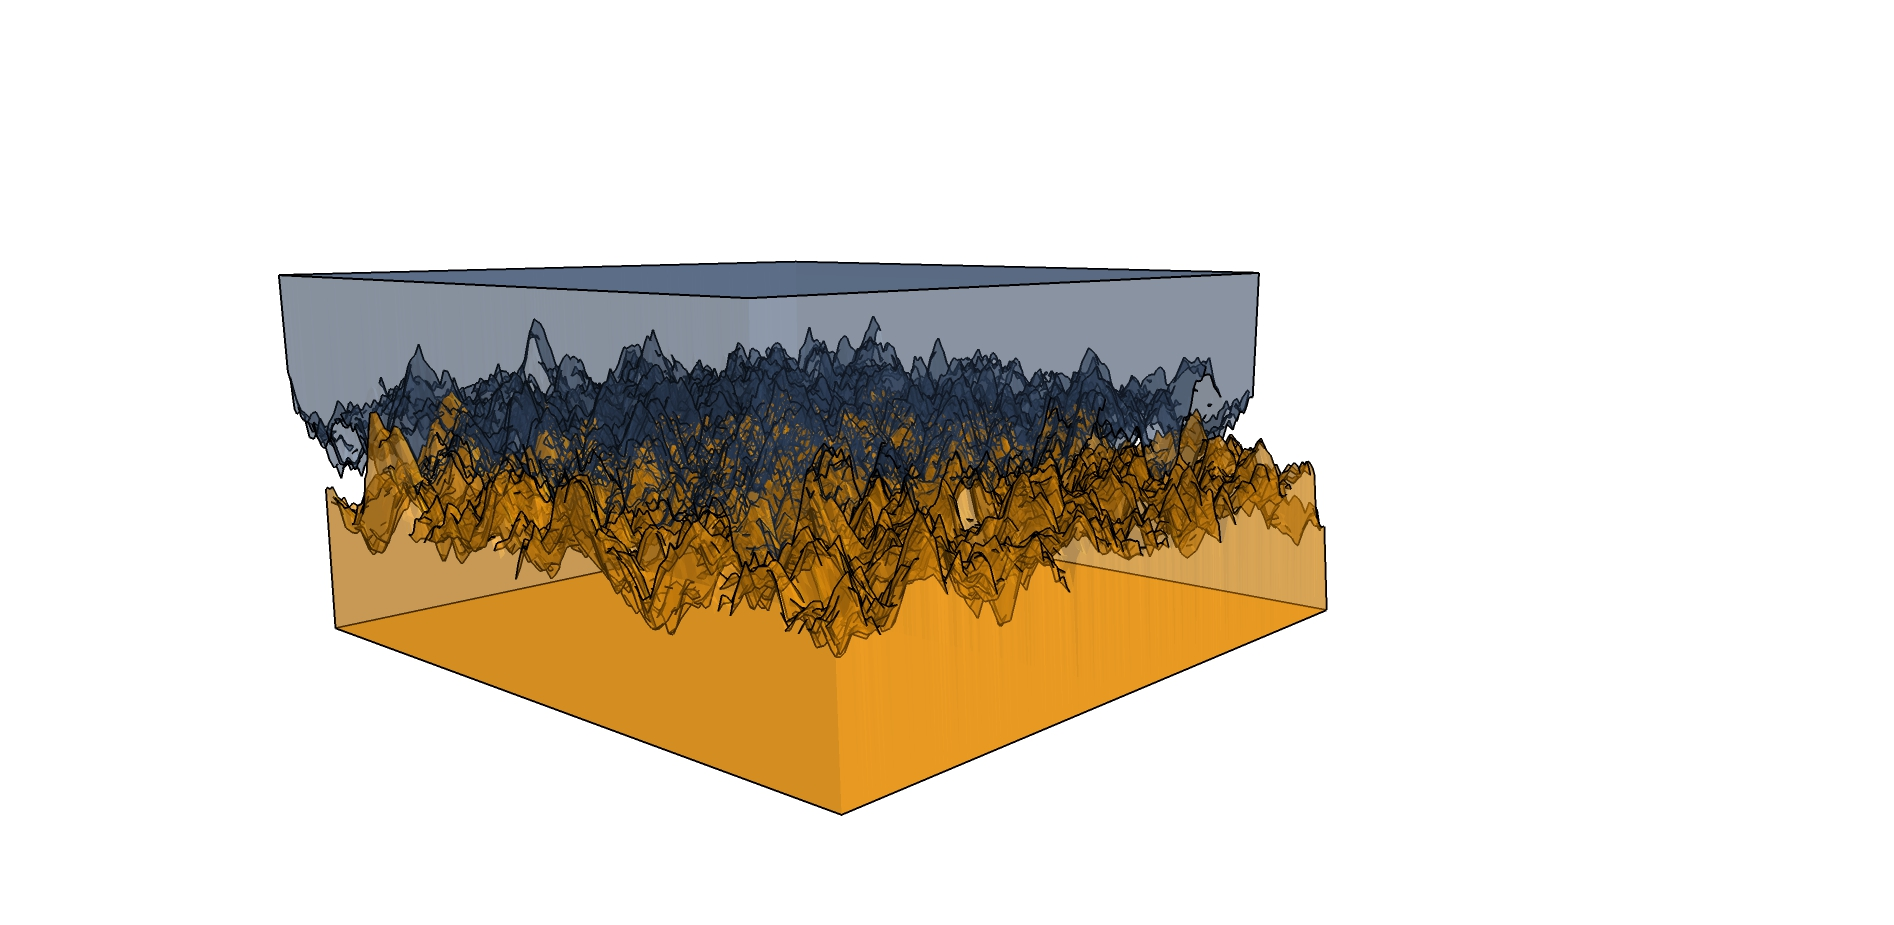
\includegraphics[width=150mm]{Friction_between_surfaces.jpg}
                        \end{adjustbox}
                        

                        \caption{Diagram showing the surface deformations that contribute to the friction forces between objects.\\Source: \href{https://commons.wikimedia.org/wiki/File:Friction_between_surfaces.jpg}{CaoHao}, \href{https://creativecommons.org/licenses/by-sa/4.0/deed.en}{CC BY-SA 4.0}}
                        \label{fig: Friction surface smoothness diagram}
                    \end{figure}

                \subsection{Normal Forces}
                    \label{subsec: Normal Forces}

                    The normal force from a surface is perpendicular to the plane of the contact (normal means orthogonal to the surface) and acts such that one object does not push through the other object.

                    The normal force of object 1 on object 2 is always equal and opposite to the normal force of object 2 on object 1.



            \newpage
            \section{Force as the Time Derivative of Momentum}
                \label{sec: Force as the derivative of Momentum}

                The definition of force as the derivative of momentum is important because in most situations it gives us the usual equation $\vect{F} = m\vect{a}$ but it also gives the correct result for situations with changing mass by giving \eqref{eq: Force with mass derivative}
                \begin{equation}
                    \vect{F} = \frac{dm}{dt}\vect{v} + m\vect{a}
                    \label{eq: Force with mass derivative}
                \end{equation}

            \section{Derivation that Net Force is Related to the Acceleration of the Centre of Mass of an Object}
                \label{sec: Centre of Mass Force Relationship}

                It is a very common assertion that the equation $\vect{F}_{net} = m\vect{a}$ is stating that the net force on an object is directly related to the acceleration of the centre of mass of the object.\\
                This is not a statement that should seem inherently true, it is often just said enough that you start to believe it.
                
                We begin by establishing that the formula for the centre of mass of an object is given by \eqref{eq: Centre of Mass Sum} (also below).\\
                This equation defines the centre of mass for a set of $N$ particles each with a constant mass.
                \begin{equation*}
                    \vect{r}_{com} = \frac{\sum\limits_{n=1}^N \vect{r}_n m_n}{\sum\limits_{n=1}^N m_n}
                \end{equation*}

                For simplicity's sake, let's set the total mass to be $M$.
                \begin{equation*}
                    \vect{r}_{com} = \frac{\sum\limits_{n=1}^N \vect{r}_n m_n}{M}
                \end{equation*}

                Taking the derivative of this equation gives the velocity of the centre of mass.
                \begin{align*}
                    \frac{d}{dt} \vect{r}_{com} &= \frac{d}{dt} \left(\frac{\sum\limits_{n=1}^N \vect{r}_n m_n}{M} \right)\\
                    \vect{v}_{com} &= \frac{\sum\limits_{n=1}^N \vect{v}_n m_n}{M}
                \end{align*}

                Taking the derivative again gives us the acceleration on the centre of mass.
                \begin{align*}
                    \frac{d}{dt} \vect{v}_{com} &= \frac{d}{dt} \left(\frac{\sum\limits_{n=1}^N \vect{v}_n m_n}{M} \right)\\
                    \vect{a}_{com} &= \frac{\sum\limits_{n=1}^N \vect{a}_n m_n}{M}
                \end{align*}

                The sum in the numerator is just the sum of all of the net forces on each particle.
                \begin{equation*}
                    M\vect{a}_{com} = \sum\limits_{n=1}^N \vect{F}_n
                \end{equation*}

                And the sum of all of the net forces is just the net force on the system as a whole. Therefore the net force on the system of particles is equal to its total mass multiplied by the acceleration on the centre of mass of the system.\\
                One particularly nice result of this is that it doesn't matter whether these particles are stuck together or not, since we haven't enforced that this condition must be true while performing the derivation.

                \begin{equation*}
                    M\vect{a}_{com} = \vect{F}_{net}
                \end{equation*}

            
            \section{Energy}
                \label{sec: Energy}

                Energy is a widely used concept in physics. Because in almost all cases energy is said to be conserved (\secref{subsec: Conservation of Energy}) it is often easier to use energy to describe what will happen rather than forces. 
                
                For example, a way of describing motion in terms of energy could be \textit{``an object falls to Earth because potential energy tends to decrease and energy must be conserved so it must lose height and gain speed.''}

                \subsection{The Law of Conservation of Energy}
                    \label{subsec: Conservation of Energy}

                    It is often outright asserted that energy is conserved in any physics problem. That \textbf{energy cannot be created or destroyed, only transformed into other types of energy}.\\
                    Mathematically this means that if you add up all of the different types of energies an object has, they should always add to the same number.\\
                    For the most part this statement is true and it's generally pretty safe to assume that it is.
                    

                    However, mathematician Emmy Noether was able to discover what is now known as Noether's Theorem which states that energy is always conserved so long as the space-time has 0 curvature. She made this discovery at the same time that Einstein was completing his work on General Relativity, the theory which describes how mass and energy curve space-time.\\
                    As a result of Noether's Theorem and Einstein's General Relativity, it cannot be said that energy is conserved on a universal scale. However, just like a small piece of a curve can be approximated as linear, a small part of space-time can be approximated as flat, so for most physics occurring on Earth, conservation of energy holds true.

                \subsection{Kinetic Energy}
                    \label{subsec: Kinetic Energy}

                    Kinetic Energy has one of the most confusing types of energy since its formula is seemingly arbitrary (\eqref{eq: Kinetic Energy}).
                    \begin{equation*}
                        E_k = \frac{1}{2}mv^2
                        \tag{\eqnum{eq: Kinetic Energy}}
                    \end{equation*}
                
                \subsection{Work}
                    \label{subsec: Work}

                    The most basic definition of work is that it is the amount of force multiplied by the distance that it acts in or, as it is regularly quoted, ``force over a distance''. For an object travelling in a straight path $\vect{s}$, with a constant force on it $\vect{F}$, the work done is the parallel component of the force multiplied by the distance (i.e. the dot product of the vectors) $W = \vect{F} \cdot \vect{s}$.

                    But how is this useful? Well, what we have to do is consider the case where the force isn't constant across the path, or where the path is not straight. In either of these cases we have to add up the infinitesimally small bits of work done along small pieces of the path $d\vect{s}$, adjusting for the changing force or path direction along the way.\\
                    The way we do this is by adding using integration, formally this type of integral is called a \textit{path integral}. From this we get the formal definition of work (\eqref{eq: Integral form of Work})

                    \begin{equation*}
                        W = \int_{\vect{a}}^{\vect{b}} \vect{F} \cdot \ud \vect{s}
                        \tag{\eqnum{eq: Integral form of Work}}
                    \end{equation*}

                    \begin{figure}[h]
                        \centering
                        \scalebox{0.8}
                        {
                            %trims left, bottom, right, top
                            \begin{adjustbox}{clip,trim=20mm 20mm 20mm 40mm}
                                {\import{images}{Work Path Integral Diagram.pgf}}
                            \end{adjustbox}
                        }
                        \captionsetup{singlelinecheck=off}
                        \caption[.]{A path followed by an object, where a small part of the path $d\vect{s}$, with the same direction as the direction of motion at that point, and a changing force $\vect{F}$.}
                        \label{fig: Work Path Integral}
                    \end{figure}
                    \FloatBarrier

                    In this case we treat the integral as a sum of infinitely many infinitesimal amounts of work done along the path (\secref{subsec: Integration as a Sum}).

                    \newpage
                    \subsubsection{Work is the change in Kinetic Energy}
                        \label{subsubsec: Work is the change in Kinetic Energy}

                        It is often asserted that the total work done on an object results in a change in Kinetic Energy of the same amount. Using the traditional (non-integral) definition of work, this can be a bit tricky to argue. However, if we assume that the mass of the object is constant (i.e. $\vect{F}_{net} = m\vect{a}$) then it is a rather simple proof.

                        First let's begin by reminding ourselves of the quantities we're dealing with:

                        \begin{align*}
                            &d\vect{s} = \Matrix{dx\\dy\\dz}\\
                            &\vect{F} = m\vect{a} = m\Matrix{a_x\\a_y\\a_z} = m\frac{d\vect{v}}{dt} = m\ \frac{d}{dt}\Matrix{v_x\\v_y\\v_z}\\
                            &\vect{v} = \frac{d\vect{s}}{dt} = \frac{d}{dt}\Matrix{x\\y\\z}\\
                            &\vect{a} \cdot \vect{b} = \vect{b} \cdot \vect{a} = a_xb_x + a_yb_y + a_zb_z
                        \end{align*}

                        We can now rearrange our equation for work using these identities.

                        \begin{align*}
                            W_{total} &= \int_{\vect{a}}^{\vect{b}} \vect{F}_{net} \cdot d\vect{s}\\
                            &= \int_{\vect{a}}^{\vect{b}} m\vect{a} \cdot d\vect{s}\\
                            &= m\int_{\vect{a}}^{\vect{b}} \frac{d\vect{v}}{dt} \cdot d\vect{s}\\
                            &= m\int_{\vect{v}_a}^{\vect{v}_b} d\vect{v} \cdot \frac{d\vect{s}}{dt}\\
                            &= m\int_{\vect{v}_a}^{\vect{v}_b} \vect{v} \cdot d\vect{v}\\
                            &= m\left(\int_{{v_x}_a}^{{v_x}_b} v_x \ud v_x + \int_{{v_y}_a}^{{v_y}_b} v_y \ud v_y + \int_{{v_z}_a}^{{v_z}_b} v_z \ud v_z\right)\\
                            &= m\left(\frac{1}{2}({{v_x}_b}^2 - {{v_x}_a}^2) + \frac{1}{2}({{v_y}_b}^2 - {{v_y}_a}^2) + \frac{1}{2}({{v_z}_b}^2 - {{v_z}_a}^2)\right)\\
                            &= \frac{1}{2}m\left(({{v_x}_b}^2 + {{v_y}_b}^2 + {{v_z}_b}^2) - ({{v_x}_a}^2 + {{v_y}_a}^2 +{{v_z}_a}^2)\right)\\
                            &= \frac{1}{2}m\left(\vmod{\vect{v}_b}^2 - \vmod{\vect{v}_a}^2\right)\\
                            &= \frac{1}{2}m\vmod{\vect{v}_b}^2 - \frac{1}{2}m\vmod{\vect{v}_a}^2\\
                            &= {E_K}_b - {E_K}_a\\
                            &= \Delta E_K
                        \end{align*}

                \subsection{Potential Energy}
                    \label{subsec: Potential Energy}

                    Potential Energy is often given the symbol $U$ and, conceptually, is the amount of work a force could to do on an object. Potential energy was invented to make conservation of energy as a law work.\\
                    Consider the case where you lift an object above your head and hold it there. While you lifted it you did work, but the object has no kinetic energy, so where did the energy go? The answer to this was potential energy.

                    Mathematically we write that the sum of the work done by a force and its potential energy are held constant at some value $E$.

                    \begin{equation*}
                        W + U = E
                    \end{equation*}
                    
                    Not all forces have an associated potential energy, typically only \textit{conservative} forces have an associated potential.\\
                    A conservative force is one where the work done by that force does not depend on the path travelled, only on the final and initial positions.\\
                    An example of a force which is not conservative is kinetic friction, since the longer your path the more distance you travel and, since it always opposes motion, it does more work. The extra lost energy here goes into other forms of energy such as heat and sound.\\
                    An example of a conservative force is gravity, since it always points in a fixed direction - down (even the spherically symmetric version is conservative but that's a little more complex for right now).

                    

                \subsection{Power}
                    \label{subsec: Power}

                    Power is the rate at which energy changes or transfers per second. Take for instance a crane lifting a load at a constant speed. Since every second it does a certain amount of work, the power being transmitted to the load is some constant value.

                    There are a few mechanisms for energy transfer, for instance heat energy ($Q$) can move between objects.
                    Work ($W$) transfers kinetic energy ($E_K$) to an object.\\
                    Since here we are considering the case of mechanical power, we will treat power as the rate at which work transfers energy to/from a system.

                    Take a small amount of work $dW$ done by a force $\vect{F}$ over a small path element $d\vect{s}$ 
                    \begin{equation}
                        dW = \vect{F}\cdot d\vect{s}
                    \end{equation}

                    Power is the derivative of work with respect to time $\left(P = \bfrac{dW}{dt}\right)$, therefore giving the result in \eqref{eq: Power vector product form}.

                    \begin{gather*}
                        P = \frac{dW}{dt} = \vect{F} \cdot \frac{d\vect{s}}{dt}\\
                        P = \vect{F} \cdot \vect{v} \tag{\eqnum{eq: Power vector product form}}
                    \end{gather*}
                    
\end{document}